%-----------------------------------------------------------------------------------
\subsection{ Hardware }

 This project implements kinematics, controls, and motion planning on a real hexapod robot platform. This platform is built of discrete components, including the hexapod hardware, sensors, and processors.

%------------------------------------------------
\subsubsection{ Hexapod }

This project uses the Freenove Big Hexapod kit as the hardware base. This kit comes with a six-legged robot chassis, where each leg has three degrees of freedom (DOF) that can be individually controlled. Each joint is actuated by an individual MG-996R servo motor, which can be commanded to move between $0-180^{\degree}$ given a 50 Hz pulse width modulation (PWM) signal. To manage communication to all 18 leg servos, the servos are controlled by the PCA9685 servo driver module, which has a standard Python library to allow software control of the PWM signals.

%------------------------------------------------
\subsubsection{ Processor }
The Raspberry Pi (RPi) 4 acts as the main processor of the robot assembly.  The RPi's CPU is a Broadcom BCM2711B0 with stock clock speeds of 1.5GHz, which has been over-clocked to 1.9 GHz for improved performance.  The model RPi used in this project includes 8MB of DDR RAM. A heat sink and active fan are used to keep CPU temperatures manageable during strenuous processing. The RPi is also setup to boot from an external SSD connected through USB 3.0, rather than the typical SD card boot hardware; this improves read-write speed and boot times.

\begin{figure}[H]
    \centerline{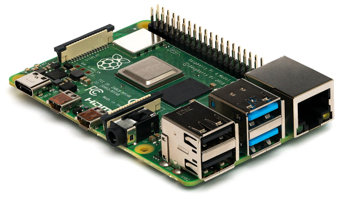
\includegraphics[scale=0.8]{04_robot_system/figures/pi1.png}}
    \caption{The Raspberry Pi 4 single-board computer}
    \label{fig:raspberry_pi}
\end{figure}

%------------------------------------------------
\subsubsection{ Seeker Gimble }

The Freenove Big Hexapod kit comes equipped with two additional sensors used for this project: an ultrasonic range sensor and a camera. These sensors are mounted together on a two-axis gimble called the ``seeker.'' The seeker can be pointed in azimuth and elevation directions individually by two MG90S servo motors, which are controlled by the RPi similar to the leg servos.

%------------------------------------------------
\subsubsection{ Raspberry Pi Camera Module}

A Raspberry Pi OV5647 infared night vision camera module is mounted to the seeker and is optimized for use with the Raspberry Pi.  It connects via a dedicated ``camera module port'' on the RPi's PCBA. It can be used for both still photos and video, and is the primary sensor for this project.

\begin{figure}[h]
    \centering
    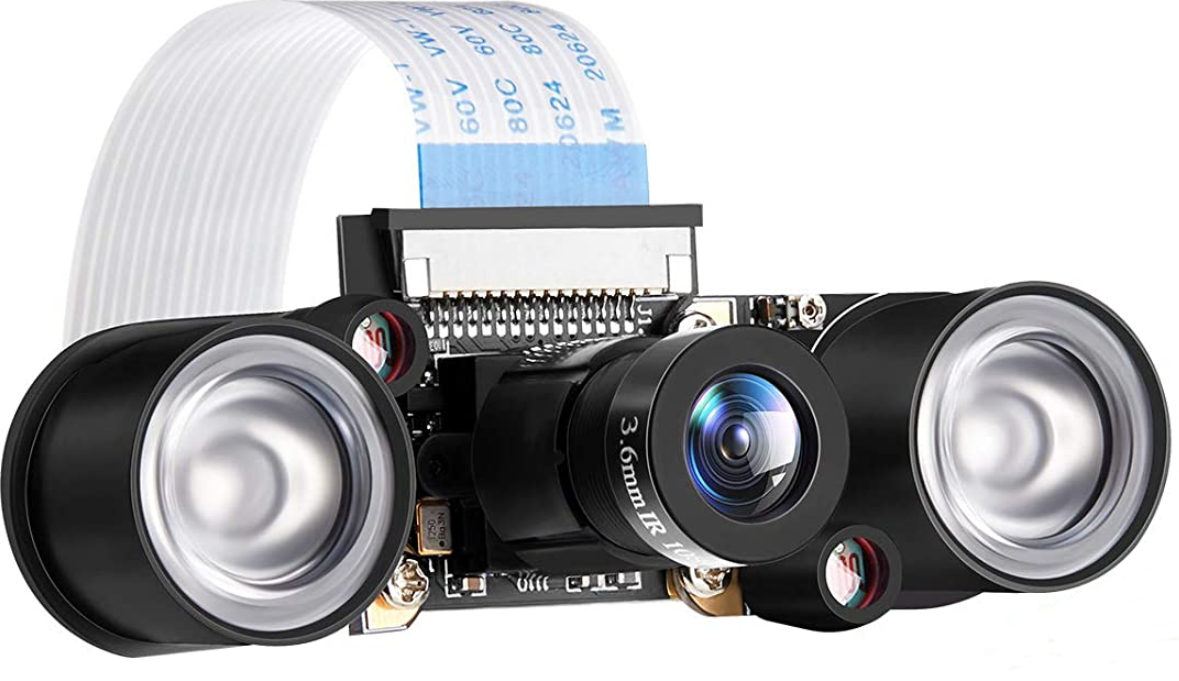
\includegraphics[scale=0.12]{04_robot_system/figures/camera.png}
    \caption{Raspberry Pi OV5647 infared nigh vision camera module}
    \label{fig:raspberry_pi_cam}
\end{figure}

%------------------------------------------------
\subsubsection{ Ultrasonic Range Sensor }
The HC-SR04 is an OTS ultrasonic range sensor mounted on the seeker and provides contactless ranging of objects from 2cm to 400cm away from the sensor \cite{hcsr04}.  The module emits a series of pulses at 40kHz that reflect on objects in front of the sensor. The sensor detects an echo reflected off an object, and the time between when the signal is sent and received can be used to estimate a range to the object. 

\begin{figure}[h]
    \centerline{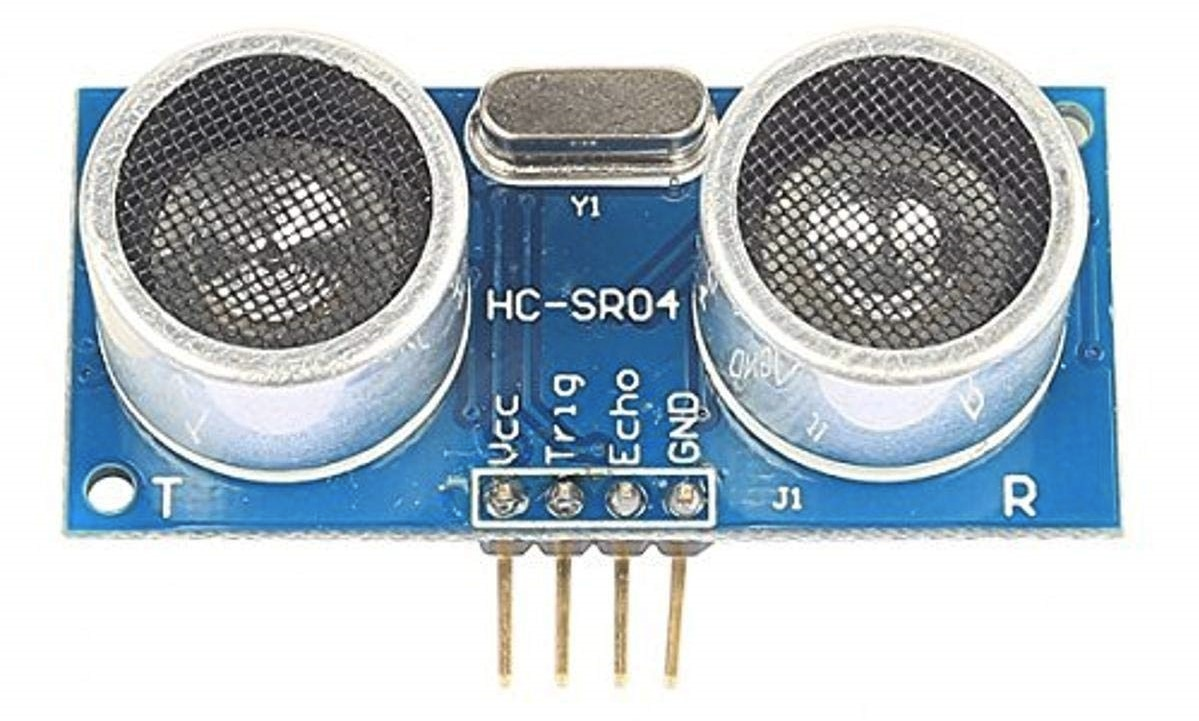
\includegraphics[scale=0.12]{04_robot_system/figures/hc_sr04.png}}
    \caption{HC-SR04 ultrasonic range sensor used on the Freenove Hexapod}
    \label{fig:HC-SR04}
\end{figure}

General purpose input-output (GPIO) pin 27 on the RPi is used to trigger the pulse, while pin 22 is used to register a detected echo. The HC-SR04's VCC and GND pins can be connected to any +5V and GND pin of the GPIO Module.

%------------------------------------------------
\subsubsection{ Inertial Measurement Unit (IMU)}
The MPU-6050 is an affordable, OTS inertial measurement unit (IMU) that is capable of providing linear acceleration, angular velocity, and temperature measurements to the Raspberry Pi at 50 Hz \cite{mpu6050}.  The IMU is hard-mounted to the motor driver board and is located just underneath the RPi. The IMU connects to the RPi via I\textsuperscript{2}C on the RPi's GPIO module.

This low-cost IMU presents inconsistent bias values for each signal which must be removed to prevent pose estimation drift. To perform this, a calibration routine was implemented in the IMU node at initialization, which assumes the robot body is static and level with the ground. The sensor is polled for some fixed time period (0.5s), and an average of all readings from both the accelerometer and gyroscope is computed. Gravitational acceleration of $9.81 m/s^2$ is removed from the $\hat{z}$ component of the accelerometer. These bias values are then removed from all future IMU measurements before publishing the data out as a ROS topic.

%------------------------------------------------
\subsubsection{ Desktop Computer }
To aleviate the computational burden of ORB-SLAM3 on the RPi, the distributed processing capabilities of ROS1 were exploited for this project by using a desktop computer to supplement the processing. This computer contained an AMD Ryzen 7 3800X 8-core CPU, an Nvidia RTX 2060 Super graphics processor, and 32Gb of onboard RAM running Ubuntu 20.04. The RPi ran all hardware-dependent ROS nodes, including the camera and IMU sensor nodes and the servo actuator nodes. All other ROS nodes, the ROS core, and any extra analysis tools, were run on the desktop machine. Communication was handled wirelessly using the local network WiFi.